\documentclass[10pt, hyperref={unicode}]{beamer}

\usepackage[czech]{babel}
\usepackage[utf8]{inputenc}
\usepackage{charter}
\usepackage{listings} 
\usepackage{xcolor} % colours
\usepackage{graphics} % pictures
\usepackage{algorithm}
\usepackage{algorithmic}
\usepackage[algo2e]{algorithm2e}
\usepackage{float}
\usepackage{multicol}

\setbeamertemplate{footline}[frame number]


\definecolor{commentgray}{RGB}{150,152,150}
\definecolor{keywordpurple}{RGB}{167,29,93}
\definecolor{stringblue}{RGB}{24,54,145}
\definecolor{blue}{RGB}{0,33,71}
\definecolor{purple}{RGB}{148,0,211}
\definecolor{darkpurple }{RGB}{106,90,205}
\definecolor{forestgreen}{RGB}{34,139,34}

\lstset{
	basicstyle=\footnotesize,
	commentstyle=\color{commentgray},
	frame=single,
	keepspaces=true,
	keywordstyle=\color{keywordpurple},
	morekeywords={new, use},
	numbers=left,
	stringstyle=\color{stringblue},
	showstringspaces=false,
	showspaces=false,
	showtabs=false,
	tabsize=4,
}
\title[Short Title]{
    Lineární vázané seznamy
    \vspace{0.5cm}
}

\author{Egor Greb\texorpdfstring{\\ xgrebe02@stud.fit.vutbr.cz}{}}
\date{\today}

\institute{
        \textit{Vysoké učení technické v~Brně}\\
        \textit{Fakulta informačních technologií}
        \vspace{0.5cm}
}

\setbeamercolor{title}{fg=blue}
\setbeamercolor{author}{fg=black}
\setbeamercolor{institute}{fg=blue}
\setbeamercolor*{subtitle}{fg=black}
\setbeamercolor*{date}{fg=black}
\setbeamerfont*{date}{size=\small}

\setbeamertemplate{title page}{
    \vspace{1cm}
    \begin{centering}
        {
        \LARGE
        \usebeamercolor[fg]{title}
        \inserttitle\\[1.5cm]
        }
        {
        \large
        \usebeamercolor[fg]{subtitle}
        \insertauthor\\[0.5cm]
        }
        {
        \small
        \usebeamercolor[fg]{subtitle}
        \insertinstitute\\[1cm]
        }
    \end{centering}
    
    \begin{flushright}
        {
        \usebeamerfont{date}
        \usebeamercolor[fg]{date}
        \insertdate
        }
    \end{flushright}
    
    \begin{picture}(0,0)
        \put(0,20){
        {\includegraphics[scale=0.1]{images/logo_cz.eps}}
        }
    \end{picture}
}

\begin{document}
\maketitle

\begin{frame}{Přehled}
	\setbeamertemplate{section in toc}[sections numbered]
	\tableofcontents[hideallsubsections]
\end{frame}




\section{Definice lineárního seznamu.}

\begin{frame}{Lineární seznam (Linked list)}
	\begin{itemize}
		\item
		Lineární seznam je \alert{dynamická datová struktura}, vzdáleně podobná poli (umožňuje uchovat velké množství hodnot ale jiným způsobem), obsahující jednu a více \textit{datových položek (struktur)} stejného typu, které jsou navzájem lineárně provázány vzájemnými odkazy pomocí \textit{ukazatelů} nebo \textit{referencí}.
				\begin{itemize}
				    \item {Každý prvek seznamu obsahuje}
				    \begin{itemize}
				        \item {Datovou část (hodnota proměnné / objekt / ukazatel na data)}
				        \item{Odkaz (ukazatel) na další prvek v seznamu.
				        \\
				        \textcolor{keywordpurple}{NULL} \textit{v případě posledního prvku seznamu.}}
				    \end{itemize}
				    \item { První prvek seznamu se zpravidla označuje jako \alert{\texttt{head}} nebo \alert{\texttt{start}}\\
				    \textit{ \footnotesize Realizujeme jej jako ukazatel odkazující na první prvek seznamu}}
			\end{itemize}
	       
	               
                \begin{picture}(100,50)
                    \put(0, 0){
                    {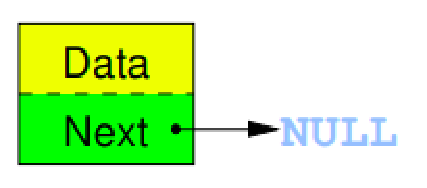
\includegraphics[scale=0.5]{images/1pic.eps}}
                }\end{picture} 
            
                      \begin{picture}(100, 50)
                    \put(100, 50){
                    {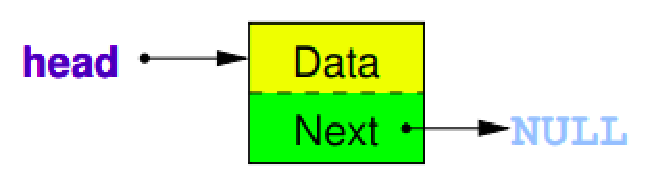
\includegraphics[scale=0.5]{images/2pic.eps}}
                }\end{picture} 
       
	\end{itemize}
\end{frame}

\section{Základní operace se spojovým seznamem.}
\begin{frame}{Základní operace se spojovým seznamem}

    \begin{itemize}
        \item {Vložení prvku}
            \begin{itemize}
                \item {Předchozí prvek odkazuje na nový prvek}
            \end{itemize}
    \end{itemize}
    
    \begin{figure}[h]
	\centering     \scalebox{0.6}{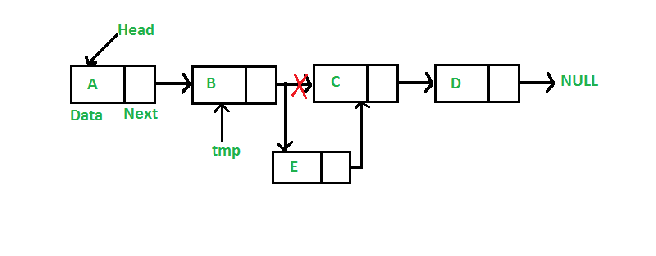
\includegraphics{images/insert.eps}}
	            \end{figure}
	            
    \begin{itemize}
        \item {Odebrání prvku}
        \begin{itemize}
            \item {Předchozí prvek aktualizuje hodnotu odkazu na následující prvek}
            \item{Předchozí prvek tak nově odkazuje na následující hodnotu, na
             kterou odkazoval odebíraný prvek}
        \end{itemize}
    \end{itemize}
    
    \begin{figure}[h]
	\centering
	\scalebox{0.6}{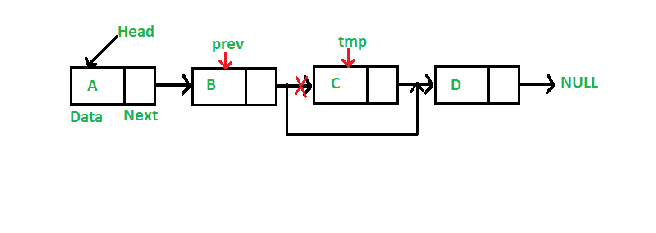
\includegraphics{images/deleting.eps}}
	  \end{figure}
\end{frame}

\section{Varianty spojového seznamu.}
\begin{frame}{Varianty spojového seznamu}
	\begin{enumerate}
		\item
			\alert{Jednosměrně zřetězený seznam}
            \begin{figure}[h]
		    \centering
		    \scalebox{0.4}{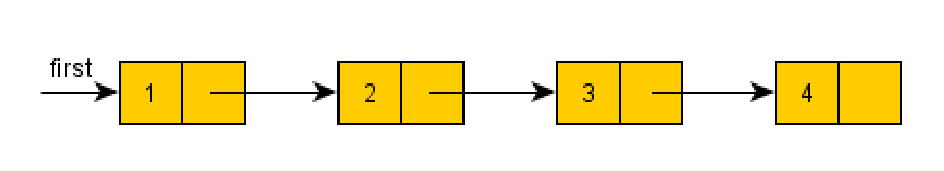
\includegraphics{images/one_direction_jpg.eps}}
	        \end{figure}
		\item
            \alert{Obousměrně zřetězený spojový seznam}
            \begin{figure}[h]
		    \centering
		    \scalebox{0.4}{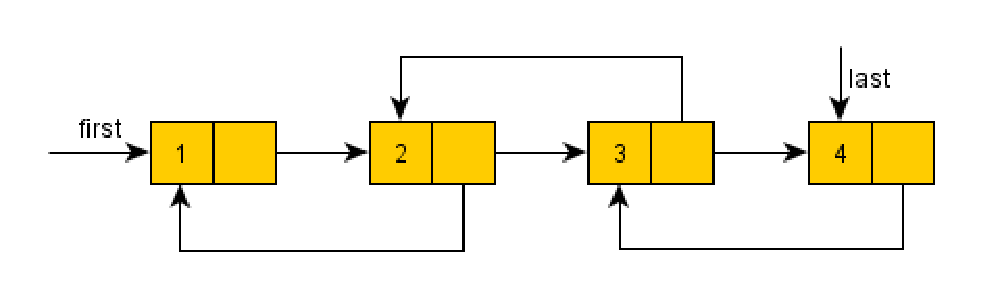
\includegraphics{images/two_direction.eps}}
	        \end{figure}
		\item
		\alert{Kruhový spojový seznam}
        \begin{figure}[h]
		    \centering
		    \scalebox{0.4}{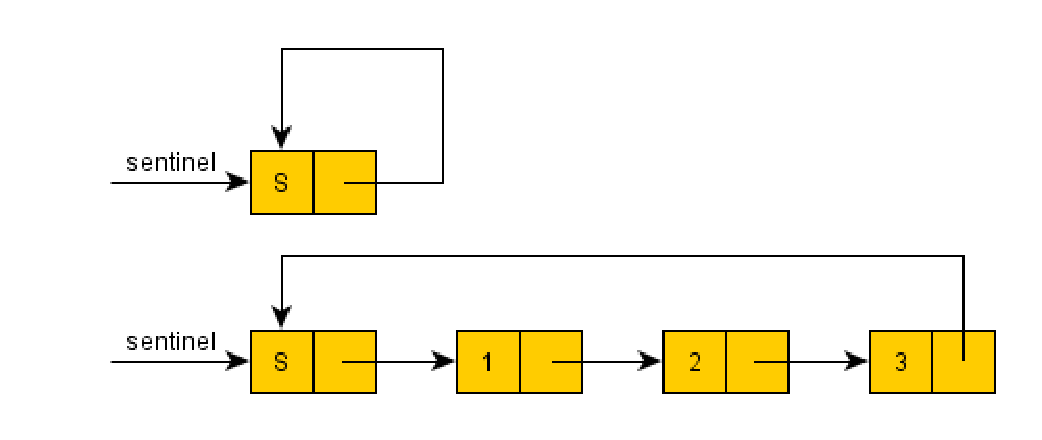
\includegraphics{images/circle.eps}}
	    \end{figure}
	\end{enumerate}
\end{frame}

\section{Ukázky pseudokódu a kódu v jázyce C pro inicializaci.}

\begin{frame}[fragile]{Seznam tvoří struktura prvku}

   \begin{itemize}
        \item Seznam tvoří struktura prvku
        \begin{enumerate}
            \item Vlastní data prvku
            \item  Odkaz (ukazatel) na další prvek
        \end{enumerate}
    \end{itemize}

    \begin{algorithm}[H]
        \text{Kód v jazyce C:} \newline
            \text{\textcolor{magenta}{typedef struct} entry \{} \newline
              \text{\textcolor{magenta}{\ \ \ \ struct} \ entry \ *next;} \newline
             \text{\textcolor{red}{\ \ \ \ int} \ value;\ \textcolor{green}{// \ data \ (celé \ číslo)}} \newline
              \text{\}\textcolor{cyan}{\ entry\_t};}
            \newline
            \newline
              \text{\textcolor{cyan}{entry\_t} \ *head = \textcolor{keywordpurple}{NULL};}
        \label{alg:seq}
    \end{algorithm}


    \hspace*{10mm}\text{\alert{Poznámka:} Pro jednoduchost prvky seznamu obsahují celé číslo.} \newline
    \hspace*{10mm}\text{Obecně mohou obsahovat libovolná data (ukazatel na strukturu).}

\end{frame}



\begin{frame}{Vlastní seznam}
    \begin{itemize}
        \item Vlastní seznam
        \begin{enumerate}
            \item Ukazatel na první prvek head
            \item Nebo vlastní struktura pro seznam \\
        \end{enumerate}
    \end{itemize}
    \hspace*{15mm}\text{\alert{\footnotesize Vhodné pro uložení dalších informací, počet prvků, poslední prvek}}

\begin{multicols}{2}

    \begin{algorithm}[H]
        \text{Pseudokód:}

        
            \textbf{Inicializace():} \newline
              $n \leftarrow 0$ \newline
              $head \leftarrow null$ \newline
              $tail \leftarrow null$
            \end{algorithm}

    \begin{algorithm}[H]
        \text{Kód v jazyce C:}

              \text{\textcolor{magenta}{typedef struct} \{} \newline
              \text{\textcolor{cyan}{\ \ \ \ entry\_t} \ *head;} \newline
              \text{\textcolor{cyan}{\ \ \ \ entry\_t} \ *tail;} \newline
              \text{\textcolor{red}{\ \ \ \ int} \ counter; \ \textcolor{green}{//počet \ prvků}} \newline
               \text{\} \textcolor{cyan}{linked\_list\_t};}

    \end{algorithm}
\end{multicols}
    
    \begin{itemize}
        \item {\texttt{n} - proměnná, aby zachovat délku struktury}
        \item {\texttt{head} - první uzel}
        \item {\texttt{tail} - poslední uzel}
    \end{itemize}
\end{frame}

\section{Názorná demonstrace metody LIFO pro praci s \textit{push} a \textit{pop}.}

\begin{frame}{Názorná demonstrace metody LIFO pro praci s push a pop}
    \begin{itemize}
        \item {LIFO je metoda manipulace s daty - data uložena jako poslední budou čtena jako první. Proto se používá také výraz LIFO z anglického „Last In – First Out“.}
    \end{itemize}

\begin{onlyenv}<1-10>
\hspace*{5mm}\includegraphics<1->[scale=0.2]{images/push1.eps}
\hspace*{6mm}\includegraphics<2->[scale=0.2]{images/push2.eps}
\hspace*{7mm}\includegraphics<3->[scale=0.2]{images/push3.eps}
\hspace*{8mm}\includegraphics<4->[scale=0.2]{images/push4.eps}
\hspace*{9mm}\includegraphics<5->[scale=0.2]{images/push5.eps}

\hspace*{5mm}\includegraphics<6->[scale=0.2]{images/pop1.eps}
\hspace*{6mm}\includegraphics<7->[scale=0.2]{images/pop2.eps}
\hspace*{7mm}\includegraphics<8->[scale=0.2]{images/pop3.eps}
\hspace*{9mm}\includegraphics<9->[scale=0.2]{images/pop4.eps}
\hspace*{9mm}\includegraphics<10->[scale=0.2]{images/pop5.eps}
\end{onlyenv}
\end{frame}

\section{Operace \textit{push}.}

\begin{frame}{Operace \textit{push}}
    \begin{itemize}
        \item Přidání prvku na začátek implementujeme ve funkci \alert{push()}
        \item Předáváme adresu, kde je uložen odkaz na start seznamu
    \end{itemize}
\hspace*{10mm}\text{\textcolor{purple}{head} je ukazatel, proto předáváme adresu proměnné, tj.} \newline
\hspace*{10mm}\text{\textcolor{purple}{\&head} a parametr je ukazatel na ukazatel} \newline
    
\text{ 
\textcolor{darkpurple }{void} push(\textcolor{red}{int} value, \textcolor{cyan}{entry\_t} **head)
} \newline
\hspace*{1mm} $\{$ \newline
\hspace*{4mm} \textcolor{cyan}{entry\_t} *new\_entry = (\textcolor{cyan}{entry\_t}*)malloc(\textcolor{darkpurple }{sizeof}(\textcolor{cyan}{entry\_t})); \newline
\hspace*{4mm} assert(new\_entry); \newline
\hspace*{4mm} \text {new\_entry} $\rightarrow$ \text{value = value;} \newline
\hspace*{5mm} \text{\textcolor{darkpurple }{if} (*head == \textcolor{keywordpurple}{NULL})} $\ \{$ \newline
\hspace*{8mm} \text{new\_entry} $\rightarrow$ \text{next = \textcolor{keywordpurple}{NULL};} \newline
\hspace*{4mm} $\} \ $ \text{else} $\ \{ $\newline
\hspace*{8mm} \text{new\_entry} $\rightarrow$ \text{next = *head;} \newline
\hspace*{4mm} $\}$ \newline
\hspace*{4mm} \text{*head = new\_entry;} \newline
\hspace*{2mm} $\}$ 
    
    \begin{itemize}
        \item Přidání prvku není závislé na počtu prvků v seznamu
    \end{itemize}
\end{frame}


\section{Operace \textit{pop}.}

\begin{frame}[fragile]{Operace \textit{pop}}

    \begin{itemize}
        \item Odebrání prvního prvku ze seznamu
    \end{itemize}  
    \textcolor{red}{int} pop(\textcolor{cyan}{entry\_t} **head) \newline
    \{ \newline
    \hspace*{4mm} assert(head != \textcolor{keywordpurple}{NULL} \&\& *head != \textcolor{keywordpurple}{NULL}); \newline
    \hspace*{4mm} \textcolor{cyan}{entry\_t} *prev\_head = *head; \newline
    \hspace*{5mm}\textcolor{red}{int} ret = prev\_head $\rightarrow$ \text{value;} \newline
    \hspace*{5mm} \text{*head = prev\_head} $\rightarrow$ \text{next;} \newline
    \hspace*{5mm} \text{\textcolor{forestgreen}{free}(prev\_head);}
    \newline
    \hspace*{5mm} \text{\textcolor{darkpurple }{return} ret;} \newline
    \}
    
    \begin{itemize}
        \item Odebrání prvku není závislé na počtu prvků v seznamu
    \end{itemize}
\end{frame}



\begin{frame}{Použité zdroje}
	\begin{thebibliography}{10}
		\bibitem[Algoritmy.net]{Algoritmy.net} Algoritmy.net		\newblock \texttt{https://www.algoritmy.net/article/24/Spojovy-seznam}

		\bibitem[Linked list, Wikipedia]{linked_list} Wikipedia: Linked list
		\newblock \texttt{https://en.wikipedia.org/wiki/Linked\_list}
		\bibitem[Stack, Wikipedia]{stack} Wikipedia: Stack (abstract data type)
		\newblock \texttt{https://en.wikipedia.org/wiki/Stack\_(abstract\_data\_type)}
	\end{thebibliography}
\end{frame}
\end{document}

